\chapter*{title}
\section{Modelo de Crecimiento Poblacional}

    **Introducción**

    Se presenta un modelo matemático para describir el crecimiento de una población de borregas, dado por la siguiente función:
    * $N(t)$ representa el número de borregas en el tiempo $t$.
    * $t$ es el tiempo en años.

    **Análisis Gráfico**

    \begin{figure}[h]
    \centering
    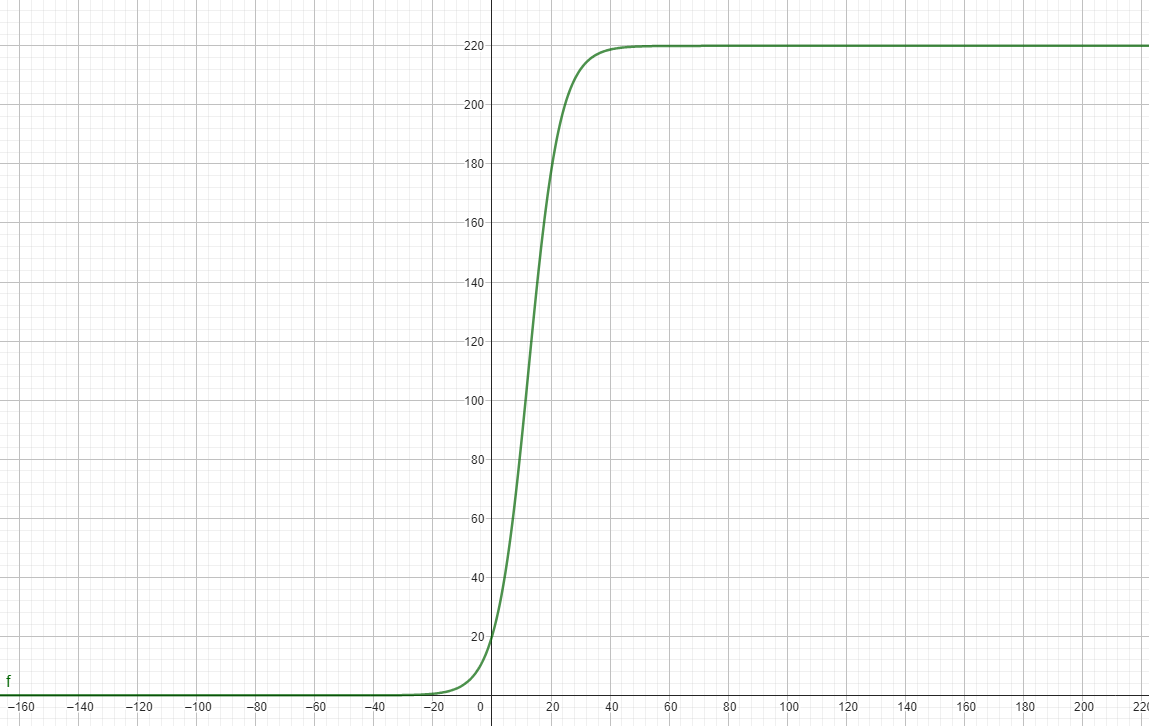
\includegraphics[width=0.6\textwidth]{matemáticas/Ejercicio13/grafica.png}
    \caption{Gráfica de la población de borregas en función del tiempo.}
    \end{figure}

    La gráfica muestra una curva de crecimiento logístico, típica de poblaciones con recursos limitados.

    **Cálculos y Resultados**

    1. **Tiempo para alcanzar 80 individuos:**

    Resolviendo para $t$, obtenemos aproximadamente $t \approx 9.36$ años.

    2. **Población máxima:**
    La población máxima que el sistema puede sostener es de 220 individuos.

    **Conclusiones**
    La población de borregas sigue un patrón de crecimiento logístico, alcanzando una capacidad de carga de 220 individuos. El modelo matemático proporciona una herramienta útil para predecir el crecimiento de la población y tomar decisiones de manejo.
